
%(BEGIN_QUESTION)
% Copyright 2006, Tony R. Kuphaldt, released under the Creative Commons Attribution License (v 1.0)
% This means you may do almost anything with this work of mine, so long as you give me proper credit

Calculate the output voltage of this op-amp circuit as the input voltage decreases (goes in a negative direction) at a steady rate of -6.5 volts per second:

$$\includegraphics[width=15.5cm]{i01524x01.eps}$$

Then, calculate the ``time constant'' of this differentiator circuit (i.e. the factor relating output voltage to input rate-of-change).

\underbar{file i01524}
%(END_QUESTION)





%(BEGIN_ANSWER)

$V_{out}$ = 0.5792 volts

\vskip 10pt

$\tau_d$ = $RC$ = 89.1 ms

%(END_ANSWER)





%(BEGIN_NOTES)

Since negative feedback from the op-amp's output holds the right-hand terminal of the capacitor at ground potential, the input voltage falling at -6.5 V/s is impressed directly across that capacitor.  We know that the current through a capacitor is described by this equation:

$$i_C = C{dv_C \over dt}$$
 

$$i_C = (0.33 \> \mu \hbox{F})(-6.5 \hbox{ V/s})$$
 

$$i_C = -2.145 \> \mu \hbox{A}$$
 
This small current, going through the 270 k$\Omega$ resistor, produces a voltage drop of:

$$V = IR$$

$$V = (2.145 \> \mu \hbox{A})(270 \hbox{ k}\Omega)$$

$$V = 0.5792 \hbox{ volts}$$
 
Since the direction of the current (conventional flow notation) is from right to left, this voltage drop across the resistor will be positive on the right and negative on the left.  With the left-hand terminal of the resistor also at ground potential (0 volts), the output voltage becomes a {\it positive} 0.5792 volts.
 
\vskip 10pt

The concept of time constant may make more sense when viewed from the perspective of {\it dimensional analysis}.  If the input rate-of-change is measured in units of {\it volts per second}, and the output (which is proportional to the input rate-of-change) is measured in the unit of {\it volts}, then the constant of proportionality must be measured in the unit of {\it seconds}:

$$\hbox{Out} = k \hbox{ In}$$

$$\hbox{[V]} = k \left({\hbox{[V]} \over \hbox{[s]}}\right)$$

$$\hbox{[V]} = \hbox{[s]} \left({\hbox{[V]} \over \hbox{[s]}}\right)$$

$k$ must be expressed in units of time (the {\it second}).

%INDEX% Electronics review: differentiator circuit

%(END_NOTES)


